\section{Modello a V}
\label{modelloV}

Il Modello a V (o V-Model) è un modello di sviluppo del software. Per la precisione si tratta di un'estensione del modello a cascata. 

\begin{figure}[H]
\centering
	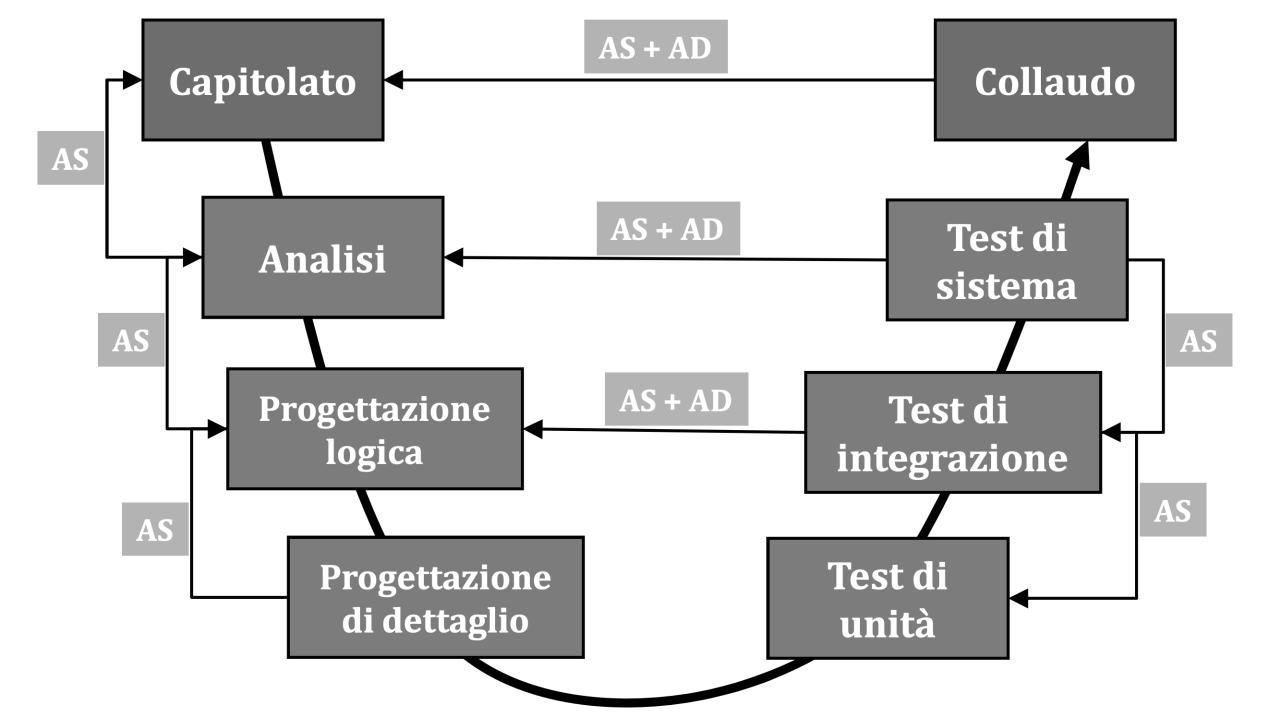
\includegraphics[width=0.7\linewidth]{./images/modellov.jpg} 
	\caption{Modello a V. Immagine dal sito web \url{https://www.math.unipd.it/~tullio/IS-1/2018/Dispense/L16.pdf}}
	\label{vmodel}
\end{figure}

Il modello a V illustra le relazioni tra ogni fase del ciclo di vita di sviluppo e la fase di testing ad essa associata. L'asse orizzontale rappresenta la completezza del progetto (da sinistra a destra); l'asse verticale il livello di astrazione (livello di astrazione minore in basso, livello di astrazione maggiore in alto).

Questo modello comprende 4 differenti livelli di test: 
\begin{itemize}
	\item \textbf{Test di Unità}: categoria di test atta a verificare la correttezza delle singole unità software. Un'unità rappresenta la più piccola componente del programma, ad esempio un metodo o una classe;
	\item \textbf{Test di Integrazione}: categoria di test atta a verificare la corretta integrazione tra le varie componenti del software. Per poter eseguire dei Test di Integrazione è necessario aver eseguito precedentemente i Test di Unità sulle varie componenti da integrare;
	\item \textbf{Test di Sistema}: categoria di test atta a verificare il soddisfacimento di tutti i requisiti, al fine di garantire che tutte le funzionalità richieste siano presenti.
\end{itemize}

